\documentclass[a4paper,12pt]{article}

\usepackage[utf8]{inputenc}
\usepackage[T2A]{fontenc}
\usepackage[russian]{babel}

\usepackage{geometry}
\geometry{left=2.5cm, right=2cm, top=2cm, bottom=2cm}

\usepackage{array}
\usepackage{multirow}
\usepackage{graphicx}
\usepackage{float}

\usepackage{caption}
\makeatletter
\renewcommand{\fnum@figure}{\normalsize Рисунок~\thefigure}
\makeatother
\captionsetup[figure]{
    justification=centering,
    font=normalsize,
    labelsep=endash,
    singlelinecheck=false
}


% Убираем номер на первой странице
\usepackage{titlesec}
\titleformat{\section}{\normalfont\large}{}{0pt}{}
\titleformat{\subsection}{\normalfont\large}{}{0pt}{}


\begin{document}

% Убираем номер на первой странице
\thispagestyle{empty}

% Страница 1

\textbf{
\begin{table}[h!]
\resizebox{\textwidth}{!}{%
\begin{tabular}{cc}
\footnotesize{Университет ИТМО}               & \multirow{3}{*}{
        
\includegraphics[width=0.25\linewidth]{logo_ITMO.pdf}
} \\
\footnotesize{Физико-технический мегафакультет} &                   \\
\footnotesize{Физический факультет}             &                  
\end{tabular}%
}
\end{table}
}

\vspace{-0.5cm}

\begin{center}
\begin{tabular}{p{0.49\textwidth}p{0.49\textwidth}}
Группа \hrulefill & К работе допущен \hrulefill \\
& \\
Студент \hrulefill& Работа выполнена \hrulefill \\
& \\
Преподаватель \hrulefill & Отчет принят \hrulefill \\
\end{tabular}
\end{center}

\vspace{1cm}

\begin{center}
    \huge{\textbf{Отчет по лабораторной работе №}} \\
    \vspace{0.5cm}
    \hrulefill\\
    \vspace{0.5cm}
    \hrulefill\\
    \textit{\small{(название лабораторной работы)}}
\end{center}

\vspace{0cm}
\textit{\hspace{9pt} Текст отчета следует печатать через один или полтора интервала, облюдая следующие размеры полей: левое — 30 мм, правое — 15 мм, верхнее и нижнее — 20 мм.
Цвет шрифта должен быть черным, размер шрифта — не менее 12 пт.
Рекомендуемый тип шрифта для основного текста отчета — Times New Roman.
Полужирный шрифт применяют только для заголовков разделов и подразделов,
заголовков структурных элементов.}

\textit{\hspace{12.5pt} При выполнении отчета необходимо соблюдать равномерную плотность и чет-
кость изображения по всему отчету. Все линии, буквы, цифры и знаки должны иметь
одинаковую контрастность по всему тексту отчета.}

\textit{\hspace{12.5pt} Страницы отчета следует нумеровать арабскими цифрами, соблюдая сквозную
нумерацию по всему тексту отчета, включая приложения. Номер страницы проставляется в центре нижней части страницы без точки.}

\section*{\hspace{30pt} Цель работы}
\vspace{1cm}

\section*{\hspace{30pt} Задачи, решаемые при выполнении работы}
\vspace{1cm}

\newpage

% Страница 2
\section*{\hspace{30pt} 1. Экспериментальный стенд \textit{(схема экспериментального стенда с пояснениями и ссылка на таблицу средств измерений, используемых в данной работе)}}

Масса каретки: \((47,0\pm 0,5)\)

\hspace{30pt} Иллюстрации (чертежи, графики, схемы, компьютерные распечатки, диаграммы, фотоснимки) следует располагать в отчете непосредственно после текста, где они упоминаются впервые, или на следующей странице (по возможности ближе к соответствующим частям текста).

\hspace{13pt} На все иллюстрации в отчете должны быть даны ссылки. При ссылке необходимо писать слово «рисунок» и его номер, например: «в соответствии с рисунком 2» и т. д.

\hspace{11.25pt} Иллюстрации следует нумеровать арабскими цифрами сквозной нумерацией. Пример оформления рисунков приведен на рисунке~\ref{fig:example}.

\begin{figure}[H]
    \centering
    
\includegraphics[width=0.25\textwidth]{example.png}
    \caption{Треугольник}
    \label{fig:example}
\end{figure}

\hspace{12.5pt} Допускается нумеровать иллюстрации в пределах раздела отчета. В этом случае номер иллюстрации состоит из номера раздела и порядкового номера иллюстрации, разделенных точкой: Рисунок 2.1.

\hspace{11.25pt} Иллюстрации при необходимости могут иметь наименование и пояснительные данные (подрисуночный текст). Слово «Рисунок», его номер и через тире наименование помещают после пояснительных данных и располагают в центре под рисунком без точки в конце.

\hspace{12.5pt} Если наименование рисунка состоит из нескольких строк, то его следует записывать через один межстрочный интервал. Наименование рисунка приводят с прописной буквы без точки в конце. Перенос слов в наименовании графического материала не допускается.

\vspace{18cm}

\newpage

% Страница 3
\section*{\hspace{30pt} 2. Обработка результатов измерений}

\subsection*{\hspace{30pt} 2.1 Результаты прямых измерений и их обработки (\textit{рабочие формулы и примеры расчетов, расчет погрешностей прямых измерений})}

\hspace{30pt}Уравнения и формулы следует выделять из текста в отдельную строку. Выше и ниже каждой формулы или уравнения должно быть оставлено не менее одной свободной строки.

\hspace{15pt}Если уравнение не умещается в одну строку, оно должно быть перенесено после знака равенства (=) или после знаков плюс (+), минус (–), умножения (×), деления(:) или других математических знаков. На новой строке знак повторяется. При переносе формулы на знаке, символизирующем операцию умножения, применяют знак «×».

\hspace{15pt}Пояснение значений символов и числовых коэффициентов следует приводить непосредственно под формулой в той же последовательности, в которой они представлены в формуле. Значение каждого символа и числового коэффициента необходимо приводить с новой строки. Первую строку пояснения начинают со слова «где» без двоеточия с абзаца.

\hspace{15pt}Формулы в отчете следует располагать посередине строки и обозначать порядковой нумерацией в пределах всего отчета арабскими цифрами в круглых скобках в крайнем правом положении на строке. Одну формулу обозначают (1). Пример оформления формул представлен на рисунке \ref{fig:formula_example}.

\begin{figure}[H]
    \centering
    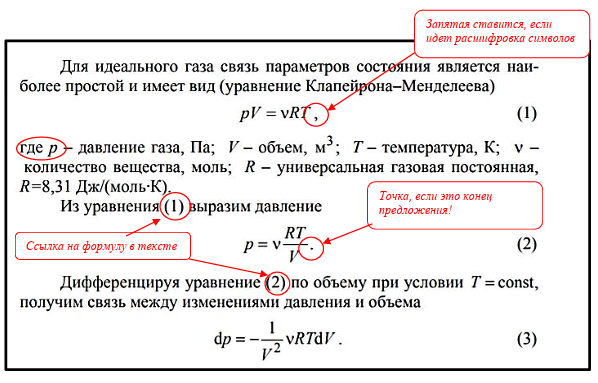
\includegraphics[width=0.80\textwidth]{formula_example.png} 
    \caption{Пример оформления формул}
    \label{fig:formula_example}
\end{figure}

\hspace{15pt}Ссылки в отчете на порядковые номера формул приводятся в скобках: в формуле~(1).

\hspace{15pt}Формулы, помещаемые в приложениях, нумеруются арабскими цифрами в пределах каждого приложения с добавлением перед каждой цифрой обозначения приложения: (В.1).

\hspace{15pt}Допускается нумерация формул в пределах раздела. В этом случае номер формулы состоит из номера раздела и порядкового номера формулы, разделенных точкой:~(3.1).

\vspace{7cm}

\subsection*{\hspace{30pt}2.2 Расчет результатов косвенных измерений (\textit{рабочие формулы и примеры расчетов, таблицы, графики, расчет погрешностей косвенных измерений})}

\hspace{30pt}Цифровой материал должен оформляться в виде таблиц. Таблицы применяют для наглядности и удобства сравнения показателей.

\hspace{15pt}Таблицу следует располагать непосредственно после текста, в котором она упоминается впервые, или на следующей странице. На все таблицы в отчете должны быть ссылки. При ссылке следует печатать слово «таблица» с указанием ее номера.

\hspace{15pt}Наименование таблицы, при ее наличии, должно отражать ее содержание, быть точным, кратким. Наименование следует помещать над таблицей слева, без абзацного отступа в следующем формате: Таблица Номер таблицы — Наименование таблицы. Наименование таблицы приводят с прописной буквы без точки в конце. Если наименование таблицы занимает две строки и более, то его следует записывать через один межстрочный интервал.

\hspace{15pt}Таблицу с большим количеством строк допускается переносить на другую страницу. При переносе части таблицы на другую страницу слово «Таблица», ее номер и наименование указывают один раз слева над первой частью таблицы, а над другими частями также слева пишут слова «Продолжение таблицы» и указывают номер таблицы.

\hspace{15pt}При делении таблицы на части допускается ее головку или боковик заменять соответственно номерами граф и строк. При этом нумеруют арабскими цифрами графы и (или) строки первой части таблицы.

\hspace{15pt}Таблицы следует нумеровать арабскими цифрами сквозной нумерацией.

\hspace{15pt}Заголовки граф и строк таблицы следует печатать с прописной буквы, а подзаголовки граф — со строчной буквы, если они составляют одно предложение с заголовком, или с прописной буквы, если они имеют самостоятельное значение. В конце заголовков и подзаголовков таблиц точки не ставятся. Названия заголовков и подзаголовков таблиц указывают в единственном числе.

\hspace{15pt}Таблицы слева, справа, сверху и снизу ограничивают линиями. Разделять заголовки и подзаголовки боковика и граф диагональными линиями не допускается. Заголовки граф выравнивают по центру, а заголовки строк — по левому краю. Горизонтальные и вертикальные линии, разграничивающие строки таблицы, допускается не проводить, если их отсутствие не затрудняет пользование таблицей.

\hspace{15pt}Текст, повторяющийся в строках одной и той же графы и состоящий из одиночных слов, заменяют кавычками. Ставить кавычки вместо повторяющихся цифр, буквенно-цифровых обозначений, знаков и символов не допускается. Если текст повторяется, то при первом повторении его заменяют словами «то же», а далее кавычками.

\hspace{15pt}В таблице допускается применять размер шрифта меньше, чем в тексте отчета. Пример оформления таблицы представлен на рисунке~\ref{fig:table_example}.

\begin{figure}[H]
    \centering
    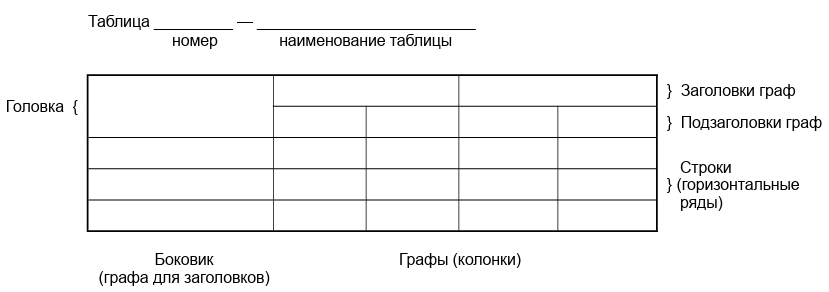
\includegraphics[width=0.9\textwidth]{table_example.png}
    \caption{Пример оформления таблицы}
    \label{fig:table_example}
\end{figure}

\hspace{15pt}Правила и примеры построения графиков и формирования таблиц приведены в методическом пособии «Обработка экспериментальных данных».

\vspace{7cm}

\newpage

% Страница 4
\section*{\hspace{30pt}3. Окончательные результаты}
\vspace{0cm}

\hspace{30pt} Пример представления окончательных результатов приведен на рисунке \ref{fig:Results}.

\begin{figure}[H]
    \centering
    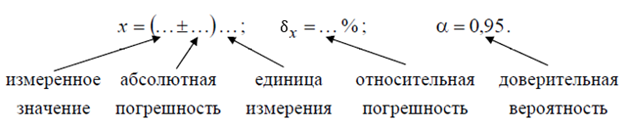
\includegraphics[width=0.9\textwidth]{Results.png} 
    \caption{Пример представления окончательных результатов}
    \label{fig:Results}
\end{figure}

\newpage

% Страница 5
\section*{\hspace{30pt} 4. Выводы и анализ результатов работы \textit{(сравнение полученных результатов с теоретическими данными, анализ полученных отклонений)}}
\vspace{18cm}

\end{document}